\documentclass{IEEEtran}

\usepackage{cite}
\usepackage{amsmath}
\usepackage{amssymb}
\usepackage{url}
\usepackage{graphicx}
\usepackage{booktabs}
\usepackage{microtype}
\usepackage[table]{xcolor}
\usepackage{tikz}
\usetikzlibrary{positioning,arrows.meta}
\usepackage[hidelinks]{hyperref}

\definecolor{networkblue}{RGB}{52,152,219}
\definecolor{envgreen}{RGB}{46,204,113}
\definecolor{algorange}{RGB}{230,126,34}
\definecolor{allocpurple}{RGB}{155,89,182}

\title{Fairness-Aware Decision-Making in Quantum Routing and Clinical Settings\\[0.3em]
{\large\textit{via Multi-Armed, Contextual, and Informative Bandit Methods}}\\[0.3em]
{\large\textit{(Approach Writeup)}}}

\author{%
\begin{minipage}{0.48\textwidth}
\begin{center}
{\bf Piter Z. Garcia}\\
\begin{small}
MS Data Science / Decision-Making \& Algorithmic Fairness\\
Rochester Institute of Technology (RIT)\\
{\it pizg8794@g.rit.edu}
\end{small}
\end{center}
\end{minipage}
\hfill
\begin{minipage}{0.48\textwidth}
\begin{center}
{\bf Dr. Daniel Krutz, Travis Desell}\\
\begin{small}
Department of Software Engineering, Data Science\\
RIT Research Advisors\\
{\it dxkvse@g.rit.edu, tjdvse@g.rit.edu}
\end{small}
\end{center}
\end{minipage}%
}

\begin{document}
\maketitle

\section{Approach Overview}
This approach writeup is designed as a direct methodological companion to the related-work
survey for the same project. The survey establishes the literature foundation, domain
motivation, and research gap; this document turns that framing into an explicit design for a
shared, reproducible evaluation framework. In both documents, the project is defined as
fairness-aware sequential decision-making across two target settings: clinical diagnostic
workflows and quantum-network routing/resource allocation. The unifying claim is that both
settings involve repeated decisions under uncertainty, partial feedback, uneven context
quality, and group-dependent risk of disparate outcomes.

The methodological focus is a spectrum of bandit methods ranging from non-contextual to
contextual to informative contextual models. This spectrum matters because the project is
not only asking which policy achieves the highest average utility, but whether richer context
reduces subgroup disparities, merely shifts them, or still requires explicit fairness-aware
mitigation. As in the survey, the clinical setting concerns sequential choices such as test
selection, triage, and follow-up escalation when patient context can be incomplete, delayed,
or noisier for some populations. Likewise, the quantum setting concerns routing and
resource-allocation decisions under probabilistic link success, scarce entanglement
resources, and changing network conditions, where service-equity gaps can emerge across
flows or user groups.

Two prior works anchor these testbeds and connect this approach directly to the survey.
First, equitable bioinformatics work provides a clinical fairness foundation and motivates
the subgroup disparity metrics used in the clinical simulation
\cite{garcia2025equitable_bioinformatics}. Second, threat-aware quantum routing work
provides the domain-realistic routing and resource-allocation foundation used for the
quantum testbed \cite{garcia2026threat_aware_quantum_routing}. The contribution is
therefore not a loose pairing of two applications, but a shared decision framework that uses
the same interaction logic, comparison spectrum, and fairness-reporting structure across
both domains.

\section{Motivating Workflows}
The survey introduces the two domains in parallel, and the approach follows that same
communication strategy by grounding the design in concrete workflows before moving to the
architecture.

\subsection{Clinical workflow}
In the clinical setting, the decision-maker repeatedly chooses actions such as ordering an
initial screen, selecting a confirmatory test, or escalating follow-up when a prior result is
ambiguous. The observed context may include patient features, prior test outcomes, sample
quality indicators, and operational constraints. However, this context may be incomplete,
delayed, or noisier for some groups, which can create subgroup differences in false
negatives, delayed escalation, or downstream care quality. The project therefore treats
clinical fairness as a time-evolving property of the sequential workflow rather than as a
single post-hoc summary of model performance.

\subsection{Quantum workflow}
In the quantum-network setting, the decision-maker repeatedly selects routes or allocates
scarce entanglement-generation attempts among competing flows. The observed context may
include link-quality estimates, queue/load signals, or threat indicators, but these inputs can
also be noisy, stale, or only partially observed. In this setting, fairness is interpreted as
service equity: whether different flow or user groups receive comparable success
probability, latency, and access to limited resources instead of having one group
consistently absorb failures or degraded service. This makes the quantum testbed a genuine
fairness setting rather than a purely performance-oriented routing benchmark.

\section{Shared Domain Model}
Figure~\ref{fig:domain_model} presents the shared architecture used to connect the two
domains.

\begin{figure*}[!t]
\centering
\resizebox{0.97\textwidth}{!}{%
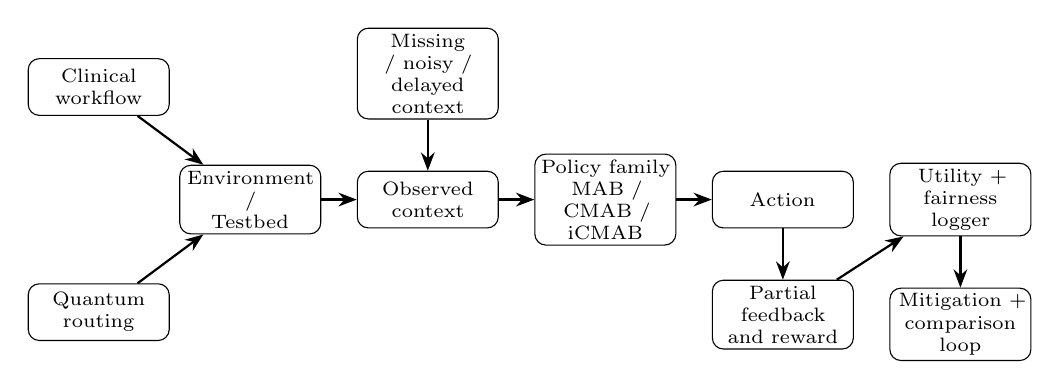
\begin{tikzpicture}[
font=\scriptsize,
box/.style={draw, rounded corners=4pt, align=center, text width=1.65cm, minimum height=0.72cm, inner sep=2pt},
arr/.style={-Stealth, thick}
]
\node[box] (env) {Environment /\\Testbed};
\node[box, above left=0.62cm and 0.12cm of env] (clin) {Clinical\\workflow};
\node[box, below left=0.62cm and 0.12cm of env] (quant) {Quantum\\routing};
\node[box, right=0.45cm of env] (ctx) {Observed\\context};
\node[box, above=0.65cm of ctx] (deg) {Missing / noisy /\\delayed context};
\node[box, right=0.45cm of ctx] (pol) {Policy family\\MAB / CMAB / iCMAB};
\node[box, right=0.45cm of pol] (act) {Action};
\node[box, below=0.65cm of act] (fb) {Partial feedback\\and reward};
\node[box, right=0.45cm of act] (log) {Utility + fairness\\logger};
\node[box, below=0.65cm of log] (mit) {Mitigation +\\comparison loop};

\draw[arr] (clin) -- (env);
\draw[arr] (quant) -- (env);
\draw[arr] (env) -- (ctx);
\draw[arr] (deg) -- (ctx);
\draw[arr] (ctx) -- (pol);
\draw[arr] (pol) -- (act);
\draw[arr] (act) -- (fb);
\draw[arr] (fb) -- (log);
\draw[arr] (log) -- (mit);
\end{tikzpicture}%
}
\caption{Shared domain model for the two testbeds. Both settings use the same fairness-aware
sequential decision architecture while retaining different operational meanings and fairness
metrics.}
\label{fig:domain_model}
\end{figure*}

The goal is to make the common sequential decision structure explicit: a testbed produces a
decision state, the system observes only the context available at that time, a policy from
the chosen method family selects an action, and the environment returns partial feedback for
that action. Utility and fairness are then logged over time and used to compare both
baseline and fairness-aware policies.

This domain model follows directly from the framing established in the survey. The two
testbeds retain different operational meanings, but the evaluation logic is shared. In both
cases, the degradation mechanism is explicit: missing, noisy, or delayed context is not an
implementation nuisance, but part of the research question. The policy family spans
multi-armed bandits (MABs), contextual multi-armed bandits (CMABs), and informative
contextual multi-armed bandits (iCMABs) so that the project can compare what happens
when the system has little context, useful context, or richer context that is still imperfect.

\section{Method Comparison Logic}
The survey argues that fairness-aware sequential decision-making must be studied under
limited context, distribution shift, and partial feedback. The approach operationalizes that
claim through a structured comparison across the method spectrum.

\subsection{Non-contextual, contextual, and informative-context methods}
A non-contextual bandit baseline provides the lowest-information comparison point. It shows
how a policy behaves when decisions are made without individual or state-specific side
information, making it useful for testing whether more context improves both utility and
fairness or only utility. A contextual policy then conditions decisions on an observed feature
vector and tests whether predictive side information improves sample efficiency and reduces
disparities. Informative-context methods extend this idea further by modeling settings where
context is richer but still subject to noise, missingness, or non-uniform quality across groups.

This spectrum matters because the project is not committed in advance to the idea that more
context is always better. In some cases, richer context may improve utility but preserve or
even amplify disparities if the context itself is unevenly available across groups. The
comparison is therefore central to the project's scientific question and keeps the approach
aligned with the survey's treatment of fairness under limited and shifting information.

\subsection{Why this design is better than simpler alternatives}
Several simpler alternatives would be easier to communicate, but they would weaken the
research contribution. A single-domain study would not test whether the same fairness-aware
decision principles remain meaningful across technically different sequential systems. A
contextual-only study would hide the central question of whether additional context actually
changes disparity outcomes relative to lower-information baselines. A post-hoc audit would
also be insufficient because the main claim of the project is that fairness must be measured
during learning under partial feedback and changing conditions. Finally, a generic framework
plus a weak transfer story would recreate the proposal problem identified in class feedback.
By contrast, the design here uses two already grounded testbeds and a shared comparison
logic, making the cross-domain structure a real research feature rather than a vague add-on.

\section{Implementation and Evaluation Plan}
The implementation plan mirrors the reproducibility and evaluation expectations already
emphasized in the survey and associated project materials. First, a clinical simulation
environment will model sequential decisions such as test ordering, retesting, or escalation
when some groups have weaker observed context. Second, the existing quantum routing
environment will represent path selection and resource allocation under probabilistic link
success, changing load, and limited quantum resources. Both testbeds will expose the same
policy interface so that MAB, CMAB, and iCMAB methods can be evaluated under a shared
logging and analysis pipeline.

The reward layer will track utility-oriented outcomes such as accuracy, cost, success rate, and
latency. The fairness layer will track domain-specific disparities such as clinical false-negative
or delayed-escalation gaps and quantum service-equity gaps in success or latency across flow
groups. This makes fairness a first-class output of the learning process rather than an
afterthought applied only at the end of an experiment.

To keep the approach credible and reviewable, experiments will run from explicit
configuration files with fixed random seeds and per-step metric logging. The simulation-first
clinical design is intentional because it allows controlled experiments under missingness,
noise, and shift without depending on sensitive patient data. The quantum testbed is
credible because it extends an existing routing and resource-allocation foundation rather than
inventing a second domain from scratch. At least one fairness-aware mitigation mechanism
will be evaluated inside the same framework so that the final comparison includes both
baseline unfairness assessment and mitigation under learning.

\section{Connection to the Survey}
The survey and this approach writeup are meant to read as two parts of the same paper and
project. The survey establishes the relevant literature on bandit methods, fairness, limited
context, clinical disparities, and quantum routing. This approach section then translates that
literature into a concrete research design with a shared domain model, parallel motivating
workflows, explicit method-spectrum comparisons, and reproducible evaluation logic. Read
together, the two documents support the same central claim: fairness-aware sequential
decision-making should be evaluated as a cross-domain problem of uneven context quality,
partial feedback, and time-evolving disparity rather than as two isolated application stories.

\begin{thebibliography}{9}\setlength{\itemsep}{0em}
\bibitem{garcia2025equitable_bioinformatics}
Garcia, P. Z. Equitable Bioinformatics: Enhancing Diagnostic Decision-Making through {RNA}
and Biomarker Data. Course paper (ISTE 780 Phase 4), Rochester Institute of Technology,
2025.
\bibitem{garcia2026threat_aware_quantum_routing}
Garcia, P. Z. Threat-Aware Evaluation of Quantum Entanglement Routing and Qubit Allocation
via Hybrid Contextual Bandits. Unpublished manuscript (GA-Work internal draft), Rochester
Institute of Technology, 2026.
\end{thebibliography}

\end{document}
